\comment{\subsection{Introduction}

Understanding how objects pack or can be designed to tile the three dimensional space is a fundamental optimization problem that has important practical applications that
range from the macroscopic, such as the efficient storage of grains,  to the microscopic: the fabrication of band-gap photonic materials.
Mathematicians have been intrigued by such problems for centuries; namely since Kepler's 1611 essay {\it On the Six-cornered Snowflakes}, but it wasn't 
until recently, with the advent of nanotechnology and the explosion of molecular biology, that problems of packing and self-assembly of nanoscopic components 
gained   tremendous traction in the broader scientific community.   
Recent advances in synthesis of nanoparticles~\cite{DeVries,Schnablegger,Hong,Weller,Hobbie,weitz,pine,mitragotri} allowed for unprecedented control over the 
 shape and surface chemistry of colloidal particles, thus providing an unlimited number of building blocks whose 
 spontaneous aggregation could lead to the formation of an unprecedented variety of structures with potentially novel functional, mechanical, and optical properties.
 Unlike most of the work on particle crystallization and self-assembly that in the last decade has focused on 
 monodisperse~\cite{frenkel1} or polydisperse~\cite{frenkel2,zaccarelli} systems of spherical or regularly-shaped particles  (see also~\cite{glotzer,chandler,geissler,cacciuto,torquato,frenkel,glotzer2,glotzer3,glotzer4,esco,weitz} and references therein), surprisingly little or nothing has been done
 theoretically to understand the packing of irregularly shaped particles. 
Indeed, there are several important cases in which the shape of the single components cannot be tailored at will,
 yet, an efficient packing, or an understanding of the physical properties of these densely compressed systems, is highly desirable.
Two examples of outstanding problems in this category are the storage of grains~\cite{deGennes} and protein crystallization~\cite{rosenberger}.
Both examples can be ideally thought of as two different aspects of the problem of understanding the role of shape in particle packing: systems of either polydisperse or indentically-shaped (monodisperse) components. 
  
Here we seek to gain insight into the crystallization of nonspherical particles. 
 We want to understand how  particle geometric features can be related to their ability to orderly pack into three dimensional periodic structures,
 and especially  to identify under what conditions they cease to do so. 
 We have recently reported~\cite{disorder1}  that it is possible to empirically relate particle geometry to crystallizability (intended as the tendency of a component to crystallize) 
by using two simple geometric parameters. The first is the particle asphericity  $A$, defined in terms of the 
surface to volume ratio of a particle $\alpha_p=A_p/V_p$ with respect to that of a sphere of diameter $\sigma$, $\alpha_s=6/\sigma$, as
$A =1-\alpha_s/\alpha_p.$  The second parameter, $q$, is related to the  orientational symmetry  of the particle.
It is used to describe the  asphericity of random walks~\cite{rudnick}, and it is obtained by combining invariants of the particle inertia tensor $I_{ij}$  as
$q=\sum_{i< j} (\lambda_i^2-\lambda_j^2)^2/\sum_i \lambda_i^2$, where $\lambda_i$, with $i=1, 2, 3$, is an eigenvalue of $I_{ij}$.
 
In this paper we try to rationalize those empirical results by computing how random perturbations from the ideal spherical 
shape affect the fluid-solid coexistence pressure of  monodisperse and shape-polydisperse systems of hard aspherical particles.

In order to generate a  statistical ensemble of aspherical particles, we developed a simple model~\cite{disorder1} that guarantees a certain degree of control over
the particle shape. Each particle is built by setting the center of $N_b$ ($4 \leq N_b \leq 12$) spheres of diameter $\sigma$ at random 
positions on the surface a spherical shell of diameter $\sigma_0<\sigma$.
The overall volume generated from the resulting overlapping aggregate defines our new particle.
Polydisperse systems of such aspherical particles were generated by choosing specific values of $N_b$ and $\sigma_0$ and allowing each particle in the system to arise from a different random collection of sphere positions.
Deviations from the ideal spherical shape can be conveniently controlled by varying $\sigma_0$ and $N_b$.
For  $\sigma_0=0$ one recovers the spherical limit, and as  $\sigma_0$ increases, particles develop larger and larger shape distortions.
In a similar fashion, large values of $N_b$ result in a bumpy but overall isotropic particle, whereas small values of $N_b$ tend to generate very anisotropic shapes.
Once a particle is built, the entire cluster is scaled so that its total volume equals that of a spherical particle of diameter $\sigma$, i.e. $\frac{\pi}{6}\sigma^3$.
Any two particles $i$ and $j$ interact via a hard repulsive potential defined as
\begin{equation}
U_{ij}=
	\begin{cases}
		0 & {\textrm{if }} |r_s-r_t|>\sigma_R \,\,\,\,\,\,\forall s\in i \,\,,\,\, \forall t\in j \cr
		\infty &\text{otherwise}\cr
	\end{cases}
\end{equation}
where $s$ and $t$ run over all spheres of rescaled diameter $\sigma_R$ constituting particle $i$ and particle $j$ respectively.
Experimental realizations of colloidal particles similar to ours could be generated using the approach described in reference~\cite{weitz,pine,mitragotri} 
to create nonspherical particles with tunable shapes. }

The results of simulations of polydisperse systems will be presented first.
Such systems could represent, for example, a system of colloidal particle which is ``sloppily'' synthesized with some tolerance for deviation from a perfect sphere.
Polydisperse systems have one major advantage, for a study such as that described below, over monodisperse systems: statistics.

In order to build up the statistical basis necessary to relate order parameters such as those described in Section~\ref{sec:asphermethod}, a large number of systems must be simulated for each data point; this severely limits the computational cost that may be expended per system.
Polydisperse systems represent a huge decrease in the number of independent variables; because each system is made up of a large number of different particle shapes, one may be confident that the result obtained is not a result of some peculiarity of a specific shape studied.
In Sections~\ref{sec:disorderpress} and~\ref{sec:disorderyesno}, monodisperse systems are studied, both as a comparison with the results attained in this section as well as using less computationally-intensive methods in order to study a larger number of particle shapes.

In order to determine the fluid-solid coexistence pressures for systems of aspherical particle, the method of direct fluid-solid coexistence simulation described in~\cite{noya} was used.
1024 particles were placed in an fcc crystal lattice (at volume density $\rho_s \simeq 0.545$, the hard sphere crystal coexistence density~\cite{HScoex}) centered in a box of dimensions $L_x \times L_y \times L_z$.
An fcc crystal was chosen based upon preliminary work, which indicated that when monodisperse aspherical systems form crystals, they tend to be (apart from a very few particular exceptions) fcc; no evidence has been found supporting the use of any other crystal geometry.

The dimensions of the box were chosen such that $L_x$ and $L_y$ were just large enough to accomodate the fcc crystal, and $L_z$ was roughly four times larger.
The crystal lattice was chosen such that the extension of the crystal in the $z$-direction was roughly twice that in the $x$- and $y$-directions, in order to increase the separation between the two fluid-solid interfaces in the system; by decreasing the surface-to-volume ratio of the crystal, one hopes to come as close to a ``bulk-like'' system as possible.

This crystal lattice was placed into equilibrium with a fluid of 1024 particles at hard sphere fluid coexistence volume density $\rho_l \simeq 0.495$.
The fluid and crystal were both briefly allowed to relax in order to relieve any overlap introduced by the ``bumpiness" of the particles and to allow the fluid to come fully into contact with the solid interface; because the particles are hard, there must be zero overlap in between particles.

Monte Carlo simulations were then run with constant number of particle $N$, pressure $p$, and temperature $T$ ($NPT$ ensemble), where the three box dimensions $L_x$, $L_y$, and $L_z$ were allowed to fluctuate independently under the isotropic pressure $p$.

The number of crystalline particles, $N_X$, in the system was monitored as a function of Monte Carlo step; this quantity was determined using the standard spherical-harmonics based bond order parameter $q_6$ described in Section~\ref{sec:orderparamdesc}.
Simulations were performed starting from a system initialized as desribed above, and $N_X$ was monitored over the course of the simulation to determine whether it decreased (crystal melting) or increased (crystal growth).

Below the coexistence pressure, the crystal will melt, and above it, the crystal will grow; thus, the pressure at which the system transitions (as a function of pressure) from decreasing $N_X$ to increasing $N_X$ represents the coexistence pressure $p^*$.
This method is known to have a few caveats: slow equilibration, non-negligible finite size effects,  dependence of the surface free energy on the specific face the crystal exposes to the fluid~\cite{noya}.
Nevertheless, for this specific system, we find this direct  method to be  more reliable than the two-step thermodynamic integration scheme described in~\cite{dijkstra}. 

\comment{\begin{figure}
	\begin{center}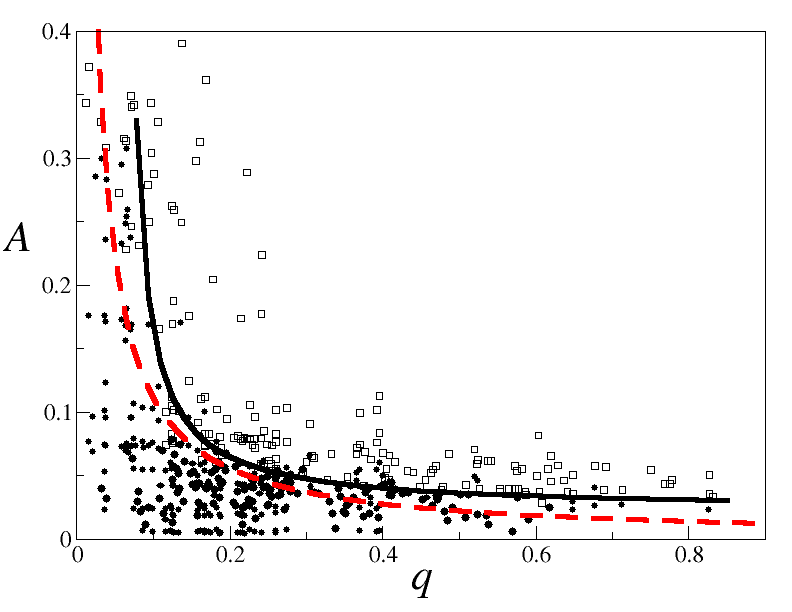
\includegraphics[width=0.8\textwidth]{polydisperse/mono1.png}\end{center}
	\caption[Crystallizability of monodispers aspherical particles vs. $A$ and $q$]{Crystallizability of monodisperse aspherical particles characterized in terms of two shape parameters $A$ and $q$. Filled circles indicate particles that easily crystallized, while open squares indicate particles that did not.  The dashed line represents a prediction of the crystallizability limit from the current work; see below.  Figure adapted from~\cite{disorder1}.}\label{mono1}
\end{figure}
Our empirical results on the crystallizability of   systems of monodisperse aspherical particles ~\cite{disorder1}, obtained by slowly compressing an ensemble of 487 different shape realizations
 are summarized in  Fig.~\ref{mono1} and indicate the existence of a clear boundary between particles that crystallize and particles that do not.
  A roughly inverse relationship is clearly evident; particles with large $A$ must have very small $q$ in order to have
a hope of crystallization, and vice-versa. This result provides a very useful way of predicting whether a particular particle shape can pack into a
crystalline structure by simply measuring the experimentally accessible $A$ and $q$. 
As this  model is intended to describe randomly shaped particles, the diagram does not include the results for particles designed with very specific shapes such as rods,
plates or regular polyhedral geometries that are known to crystallize. 
These particular cases would generate sharp peaks around specific values of $q$, and are purposefully excluded from this study.
 The solid line is  a guide to the eye and has the functional form $A(q) = 0.023 + 1/(170q-10)$.} 

Incorporating shape-polydispersity in these systems is not a trivial matter and requires some discussion.  
Unlike the common notion of polydispersity of spherical particles  for which any particle size can be indifferently used as a reference (and thus only the width, not the center, of the distribution matters), each particle shape could be used as a reference shape for this study. 
The problem is that the phase behavior could be very much dependent on the specific choice of $A$ and $q$.
We therefore adopted a pragmatic approach to describing shape-polydispersity  that has a natural experimental counterpart~\cite{weitz}. 

\begin{figure}
	\begin{center}
		\subfloat[]{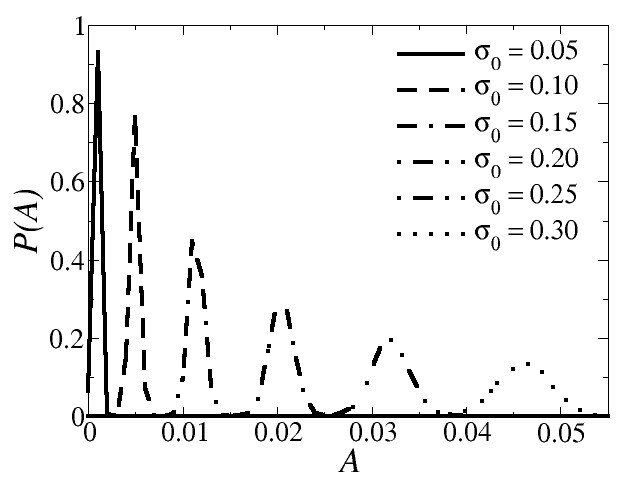
\includegraphics[width=0.6\textwidth]{polydisperse/Ahist.png}\label{Ahist}}

		\subfloat[]{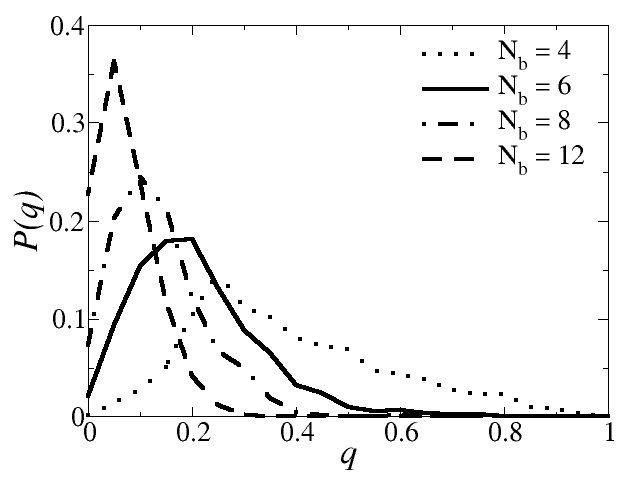
\includegraphics[width=0.6\textwidth]{polydisperse/qhist.png}\label{qhist}}
	\end{center}
	\caption[$A$ and $q$ distributions for different values of $\sigma_0$ and $N_b$]{\subref{Ahist} Probability distributions of $A$ for polydisperse systems with $N_b = 8$ and various values of $\sigma_0 \in [0.05,0.30]$.  the $A$ distribution is approximately independent of $N_b$.  \subref{qhist} Distribution of $q$ values for polydisperse systems with $N_b$ = $4$, $6$, $8$, and $12$.  Recall that $q$ is independent of $\sigma_0$.  The distribution is significantly larger and broader for $N_b = 4$ than for the larger values of $N_b$.}\label{histograms}
\end{figure}

Namely, we  consider the distributions of $q$s and $A$s arising when constructing our particle using a given number of spheres $N_b$ and a given value of $\sigma_0$.
Particles  with large values of $N_b$ generate narrow distributions shifted towards small values of $q$, while small values of $N_b$ ($N_b\geq 4$) result in wide distributions peaked over large values of $q$.
When $\sigma_0\rightarrow 0$ one recovers the  hard sphere limit for any value of $N_b$, and as $\sigma_0$ increases,  larger and larger values of $A$ will be sampled (without affecting the $q$ distributions) until approaching the crystallizability boundary.
Sample distributions of $A$ and $q$ for varying values of $\sigma_0$ and $N_b$ (respectively) are shown in Figure~\ref{histograms}

We systematically analyzed particles constructed with $N_b =4$, $5$, $6$, $8$, and $12$, and values of  $\sigma_0 \in[0.05,0.30]$.

\begin{figure}
	\begin{center}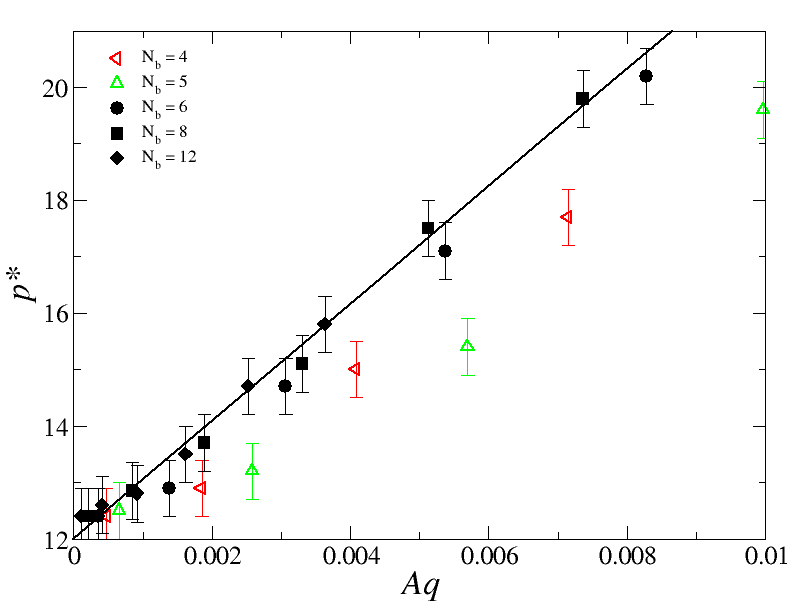
\includegraphics[width=0.8\textwidth]{polydisperse/poly.png}\end{center}
	\caption[Coexistence pressures for shape-polydisperse systems vs. $Aq$]{Coexistence pressure vs. $Aq$ for shape-polydisperse systems of hard aspherical particles. The solid line is a fit to the data for $N_b\geq 6$.}\label{poly}
\end{figure}
All data points have been computed using two different random sets of particle geometries from the given distribution.
The difference between the results from the two independent sets is smaller than the error bar associated with the numerical scheme.
Figure~\ref{poly} shows our results: the coexistence pressure $p^*$ (as defined above) versus the product $Aq$ for $4 \leq N_b \leq 12$ and $\sigma_0 \in [0.05,0.30]$.

Unsurprisingly, the coexistence pressure increases with increasing $A$ and $q$, but remarkably, for $N_b \geq 6$, the relationship between $p^*$ and $Aq$ is simple linear one.
We find that the coexistence pressures for these $N_b$ values  be fitted to  $p^* (A,q)= 991Aq + 12$.
Note that the y-intercept is near the hard sphere coexistence pressure of $p^*_{\rm HS}\simeq  11.7$~\cite{HScoex}, as it should be.
This should be expected because the $Aq \rightarrow 0$ limit is a system of hard spheres.

These results thus suggests that $p^*(A,q)$ can be expressed in terms of a Taylor expansion in the quantity $Aq$: 
\begin{equation}
	\frac{p^*(A,q)-p^*_{\rm HS}}{p^*_{\rm HS}} = \alpha Aq + ...
\end{equation}
Note, however, that significant but systematic deviations from the linear fit are visible for systems of particles obtained with  $N_b = 4$ and $N_b = 5$. 
These values of $N_b$ correspond to particles with  relatively large values of $q$ and rather broad distributions (see Figure~\ref{qhist}), suggesting that other, higher-order terms in the expansion may be necessary. 
Furthermore, for such wide distributions fractionation  between isotropic and anisotropic particles may become an important factor -- this is an effect to which the direct simulation method used here is completely blind, because the system is initialized with a preformed crystalline volume with a random selection of particles.
Fractionation would require complete melting of the initial crystal and subsequent formation of a fractionated crystal, which was not allowed in this study.
